\documentclass[10pt,twocolumn]{article}
\usepackage[margin=0.72in]{geometry}
\usepackage{graphicx}
\usepackage{booktabs}
\usepackage{amsmath}
\usepackage{hyperref}
\usepackage{url}
\usepackage{microtype}
\usepackage{caption}
\usepackage{enumitem}
\graphicspath{{figures/}}
\setlength{\columnsep}{0.22in}
\setlength{\parindent}{1em}
\setlength{\parskip}{0pt}
\title{Visibility Is Not Detection: Auditing Measurement Boundaries in Staged and Evidence-Ranking Evaluation}
\author{Author TBD\_OWNER\\Affiliation TBD\_OWNER\\Corresponding author TBD\_OWNER}
\date{Submission package draft; owner fields intentionally marked TBD\_OWNER}
\begin{document}
\maketitle
\begin{abstract}
\noindent\textbf{Purpose:} We audit whether reported evaluation scores distinguish observed defects from silent absorption and whether evidence-ranking conclusions survive implementation choices. \textbf{Methods:} We retain the original two-case scope: a frozen staged document evaluator with controlled header perturbations, instrumentation and a nested FinQA measurement-object probe; and FinRank, a public provenance-sensitive evidence-ranking benchmark. We inspect visibility, detection, harmfulness, score algebra, tie policy, identity construction, and reproduction. \textbf{Results:} In the staged case, 96/118 header injections are visible, the OCR-like family is unobserved on the frozen surface (0/13), and flat versus layered scores are affine/rank-equivalent. Explicit instrumentation explains stage separation, while clean-only calibration does not identify a deployment threshold. In FinRank, tie policy changes absolute metrics but preserves the hard-versus-random direction; a post-hoc text-sha1 correction finds 442 overlapping hard-negative occurrences across 305 records and gold loss in 33 records. In-record and pairwise values reproduce exactly, but global and metadata-filtered drift remains unexplained. \textbf{Conclusion:} The two cases support a bounded review discipline: bind observations to measurement objects, separate score sensitivity from decision stability, preserve identity contracts, and report unresolved reproduction gaps. We do not claim a universal causal theory, formal acceptance, or generalization beyond these cases.
\end{abstract}

\section{Introduction}
Final-answer scores can hide whether an evaluation observed a defect, consumed the observation, or treats the outcome as harmless. We therefore separate visibility, detection, contract-relative harmfulness, score sensitivity, decision stability, and reproduction gap. This paper retains the existing two-case scope and does not add C2/C3 experiments. Figure~\ref{fig:chain} summarizes the measurement chain.

\begin{figure}[t]
\centering
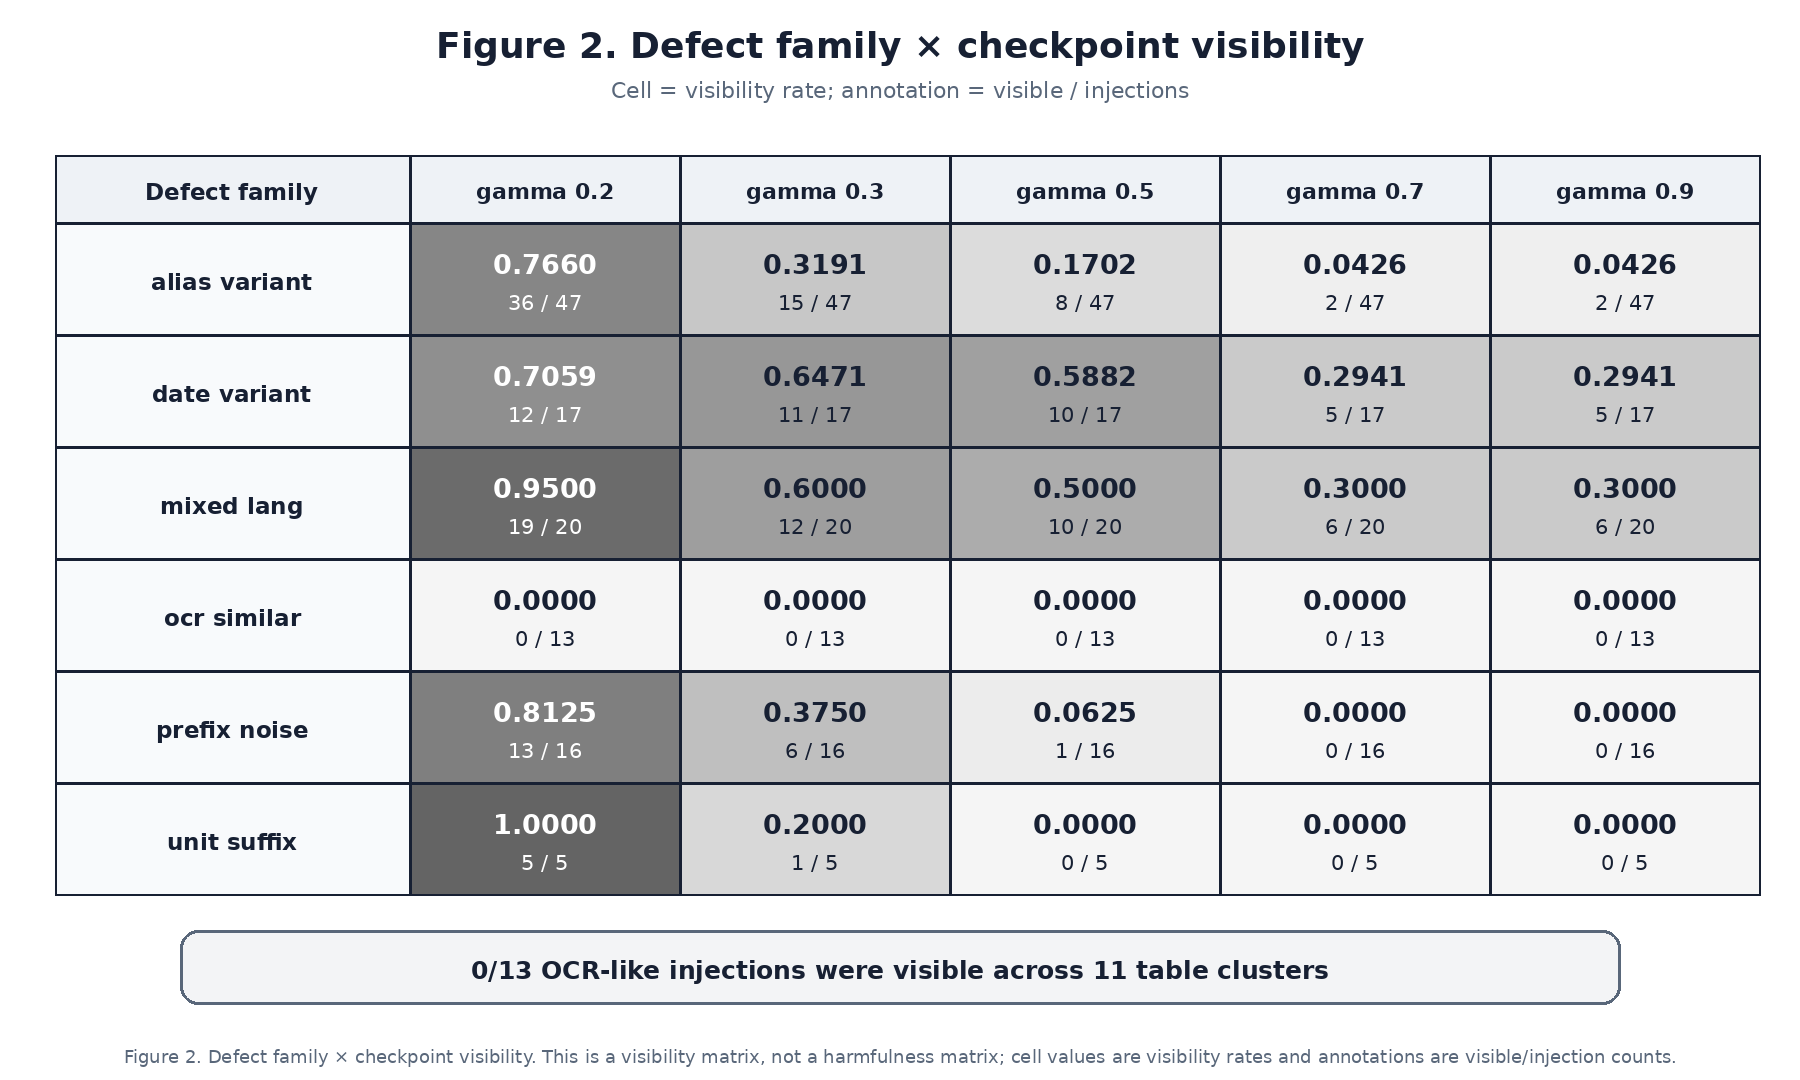
\includegraphics[width=\columnwidth]{fig2_family_visibility_matrix.png}
\caption{From injected failure to visibility, protocol detection and contract-relative outcome harm.}
\label{fig:chain}
\end{figure}

\section{Two Audited Cases}
\subsection{Case 1: staged document evaluator}
The staged evaluator reports 96/118 visible header injections and 0/13 OCR-like observations on the frozen surface. Harmfulness is contract-relative rather than an intrinsic property of a perturbation. Flat and layered score constructions are affine/rank-equivalent, so their apparent agreement is not independent validation. Explicit stage instrumentation explains the perfect stage separation; a clean-only panel cannot identify the deployment threshold. A nested FinQA probe tests whether perturbation and detection predicates refer to aligned measurement objects; it is not treated as a new downstream result.

\subsection{Case 2: FinRank}
The FinRank audit separates tie policy from the hard-versus-random ordering. Reversing tie priority lowers MRR and nDCG@5, while the qualitative ordering remains stable. The identity branch is explicitly post-hoc v2: a canonical \texttt{text\_sha1} correction finds 442 overlapping hard-negative occurrences across 305 records and gold loss in 33 records. These are corrections to this audit's identity implementation, not corrections to FinRank. In-record and pairwise values reproduce exactly; global and metadata-filtered values drift by up to 0.19 and 0.16 points in the declared environment, with residual cause unresolved.

\begin{figure}[t]
\centering
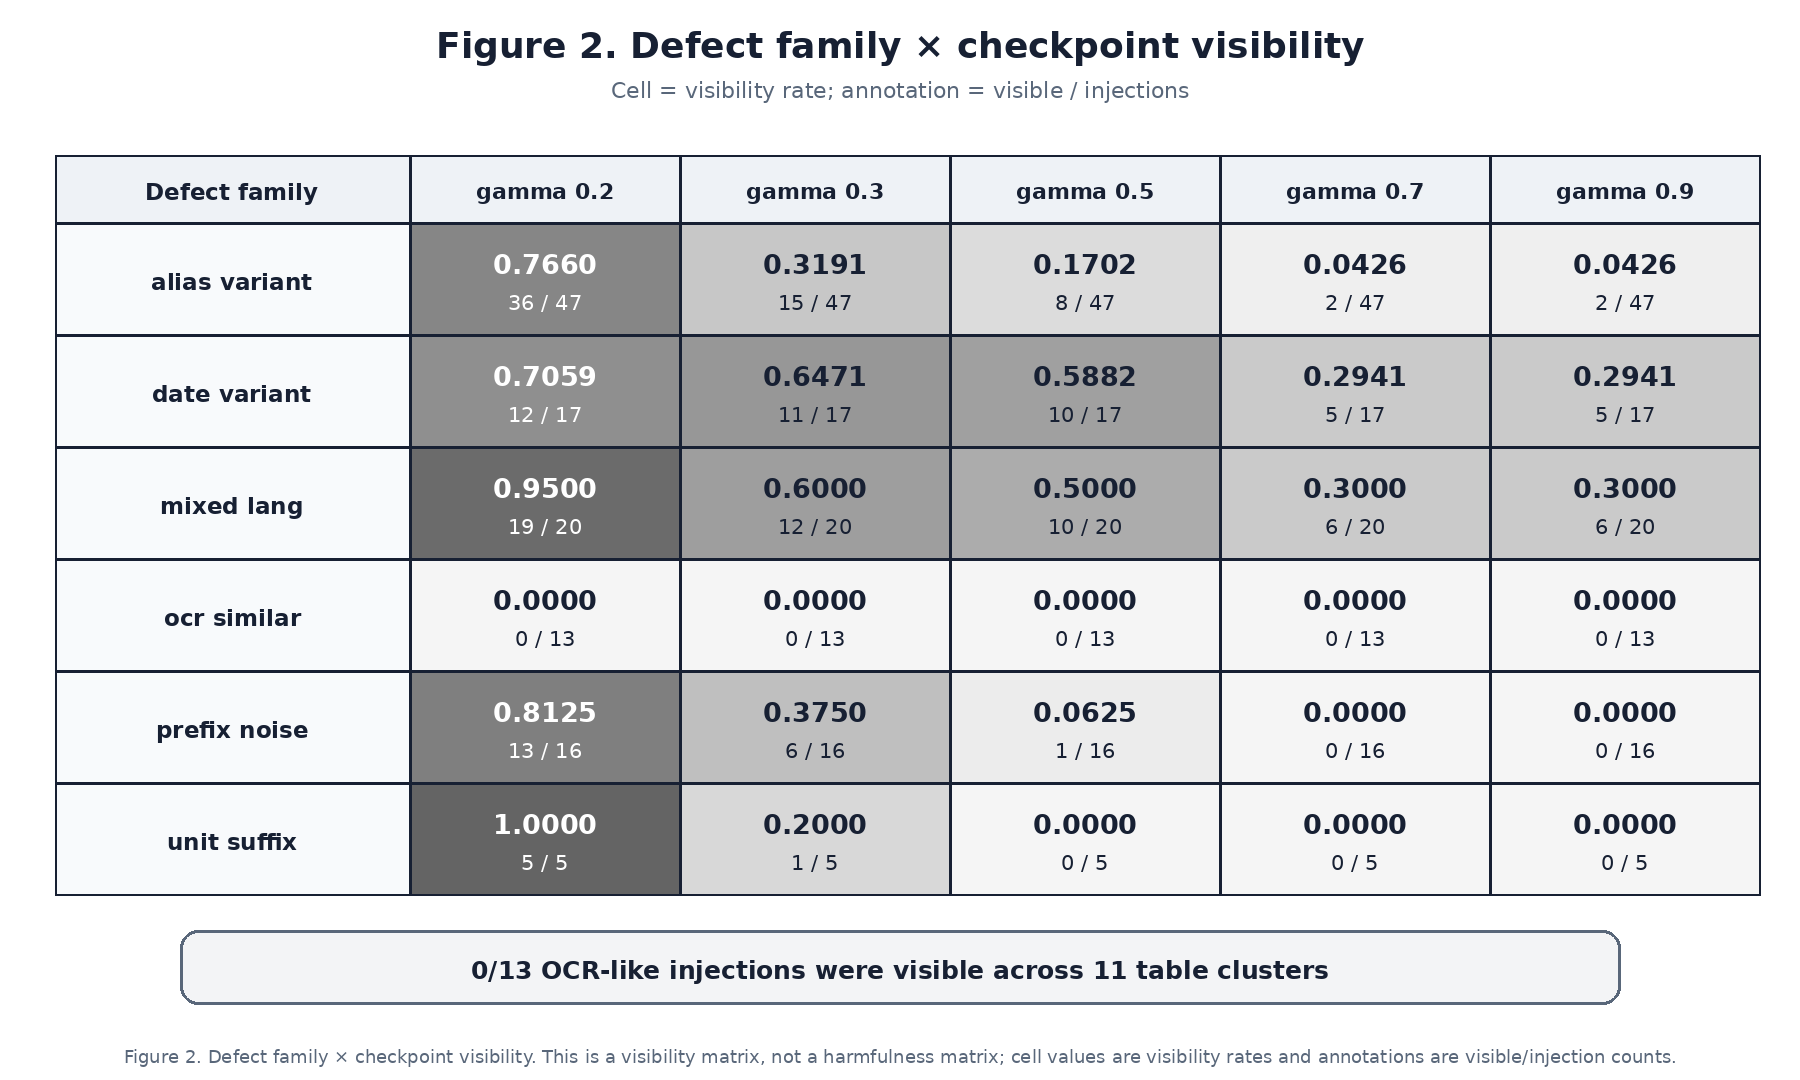
\includegraphics[width=\columnwidth]{fig2_family_visibility_matrix.png}
\caption{Family-dependent visibility matrix from the staged evaluator.}
\label{fig:visibility}
\end{figure}

\begin{figure}[t]
\centering
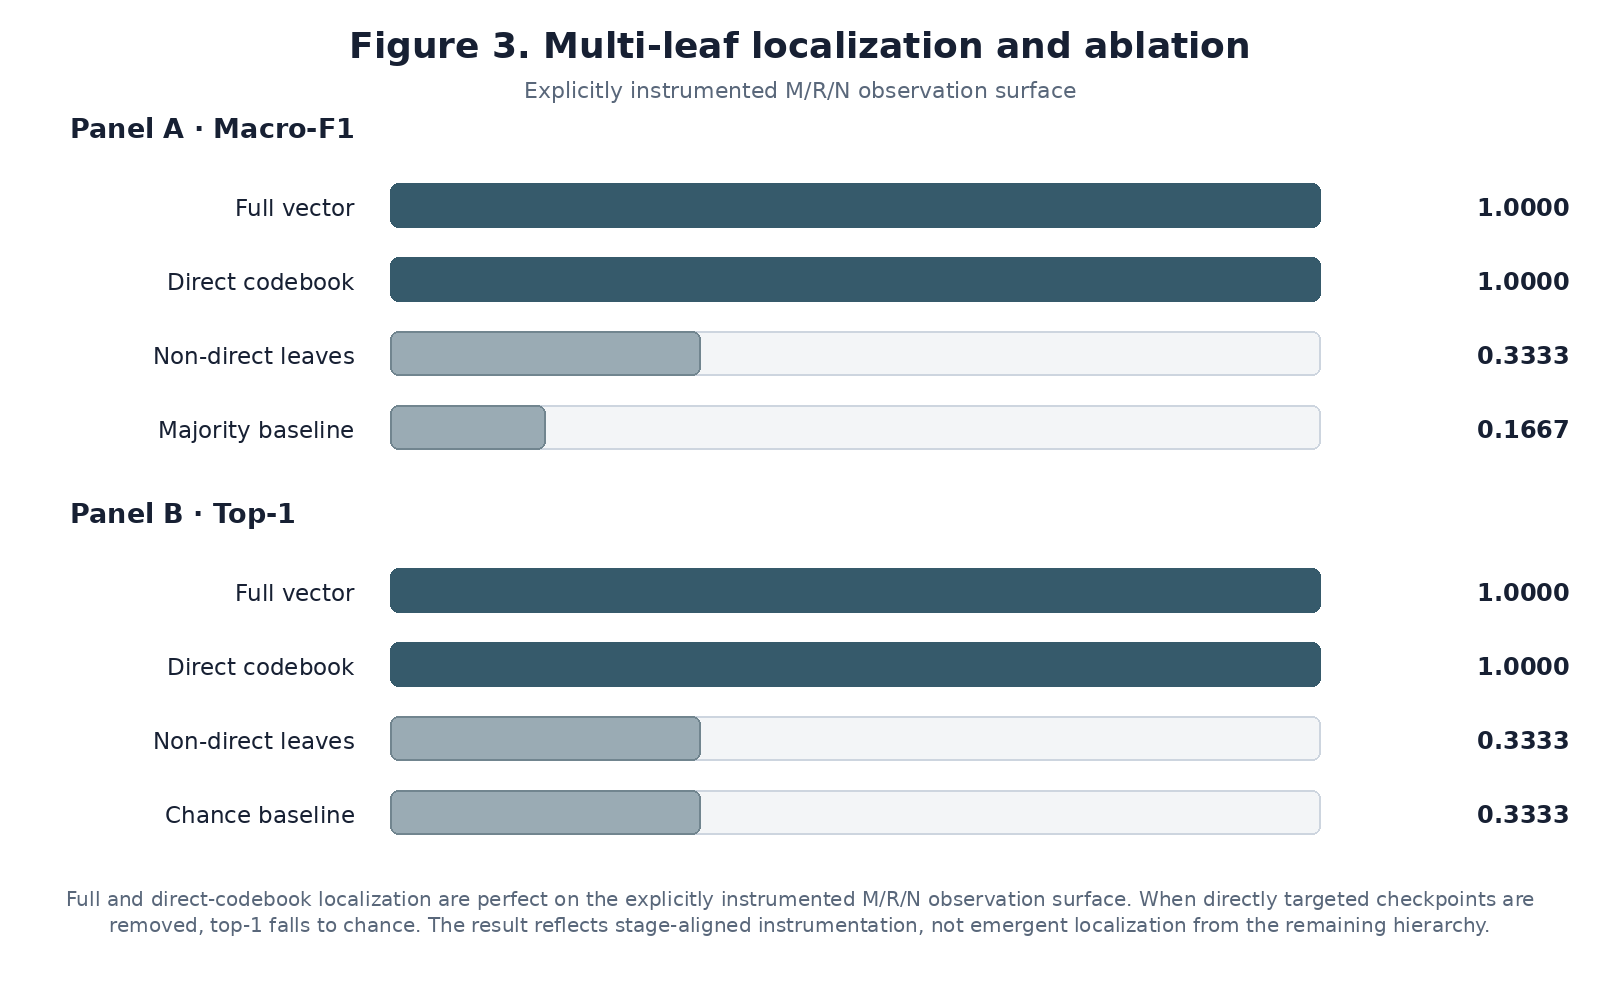
\includegraphics[width=\columnwidth]{fig3_localization_ablation.png}
\caption{Localization ablation used in the staged evaluator audit.}
\label{fig:ablation}
\end{figure}

\section{Reviewer Pass}
The contribution boundary is an audit discipline, not a new evaluator or ranking method. The closest work includes measurement-validity and reproducibility practice, but the bounded novelty here is the explicit separation of six objects and the paired, case-specific evidence. The FinRank identity correction is post-hoc and clustered by canonical text identity; it must not be read as a second frozen application. The two cases changed the interpretation of score agreement and the status of identity-sensitive counts, but they do not establish a natural failure distribution or causal mechanism. Unexplained items remain: why OCR-like injections are invisible on this surface, whether other tie policies would change deployment decisions, and whether global/metadata metric drift is caused by dependency, serialization, or ordering.

\section{Limitations}
Case 1 uses synthetic perturbations on one public corpus; Case 2 covers TF-IDF and BM25 rather than neural or generative systems. The semantic boundary analysis uses one judge on 28 cases. The post-hoc identity correction is not preregistered. Neither case supports claims of acceptance, publication, school recognition, or generalization.

\section{Conclusion}
A defensible evaluator audit should bind perturbations to measurement objects, inspect score algebra and tie policy, preserve source identity, test decision stability, and report reproduction boundaries. The evidence supports this checklist as a proposed discipline, not as a validated universal method.

\begin{thebibliography}{9}
\bibitem{nist}
National Institute of Standards and Technology.
\newblock \emph{AI Risk Management Framework}, 2023.
\bibitem{tatqa}
Zhu et al.
\newblock TAT-QA: A question answering benchmark on a hybrid numerical-textual database.
\newblock \emph{ACL}, 2021.
\end{thebibliography}
\end{document}
